\chapter{Operating the Decision-Support System}
\section{A short operator workflow}
\begin{enumerate}
\item Identify the line in \textbf{RAG > Devices}; the UI has no dedicated manufacturing-line selector. State dataset code \texttt{ZSK-SIM-01} explicitly and resolve its relationship to RAG \texttt{ZSK-001} before combined analysis.
\item Ask chat to retrieve recent stored measurements and previous comparable recipe conditions. Check timestamps/units; September synthetic readings are not current October telemetry.
\item Request analysis/prediction. Review label, probability, history/warmup and model version; a Healthy label is not an operating-safety clearance.
\item Inspect supporting passages in \textbf{RAG > Knowledge Search} and document/chunk details in \textbf{Documents}. Ranking is not confidence. Chat \textbf{+} attachments are local files, not searchable RAG ingestion.
\item Ask for observations, model result, source evidence, interpretation, inspection priority and uncertainty separately. Treat possible causes as hypotheses.
\item Expand chat tool activity or task \textbf{Requests and outputs}; review the exact call/results. Physical inspections and maintenance decisions remain with the operator and qualified technician.
\end{enumerate}
\section{Example prompts and task recovery}
``What is the current health status of ZSK-001? First verify its dataset identity and data freshness.'' ``Analyze the gearbox vibration trend and explain possible causes using the available documentation.'' ``Compare the latest measurements with previous operating conditions.'' ``What inspection should the operator prioritize based on the available evidence?'' Include the verified dataset code once known; do not instruct the model to guess the mapping.

Check \textbf{Run as task} before Send for durable work, or use \textbf{TASKS > Active Tasks > New task}. Monitor the live card; \textbf{View task details} opens plan, Completion checks, Verification evidence and Tool execution history/Request and result. PAUSED uses \textbf{Resume}; FAILED uses \textbf{Retry}. Resolve pending \textbf{Approve action/Reject action} and \textbf{Reconcile outcome} first. Ordinary chat uses \textbf{Confirm and run/Decline} and \textbf{Retry response}. Cancellation preserves past effects. ``100\% verified'' means task predicates passed; response-only completion explicitly verifies no external operation. Scheduled Tasks supports cron/one-time execution; there is no trigger control.
\begin{center}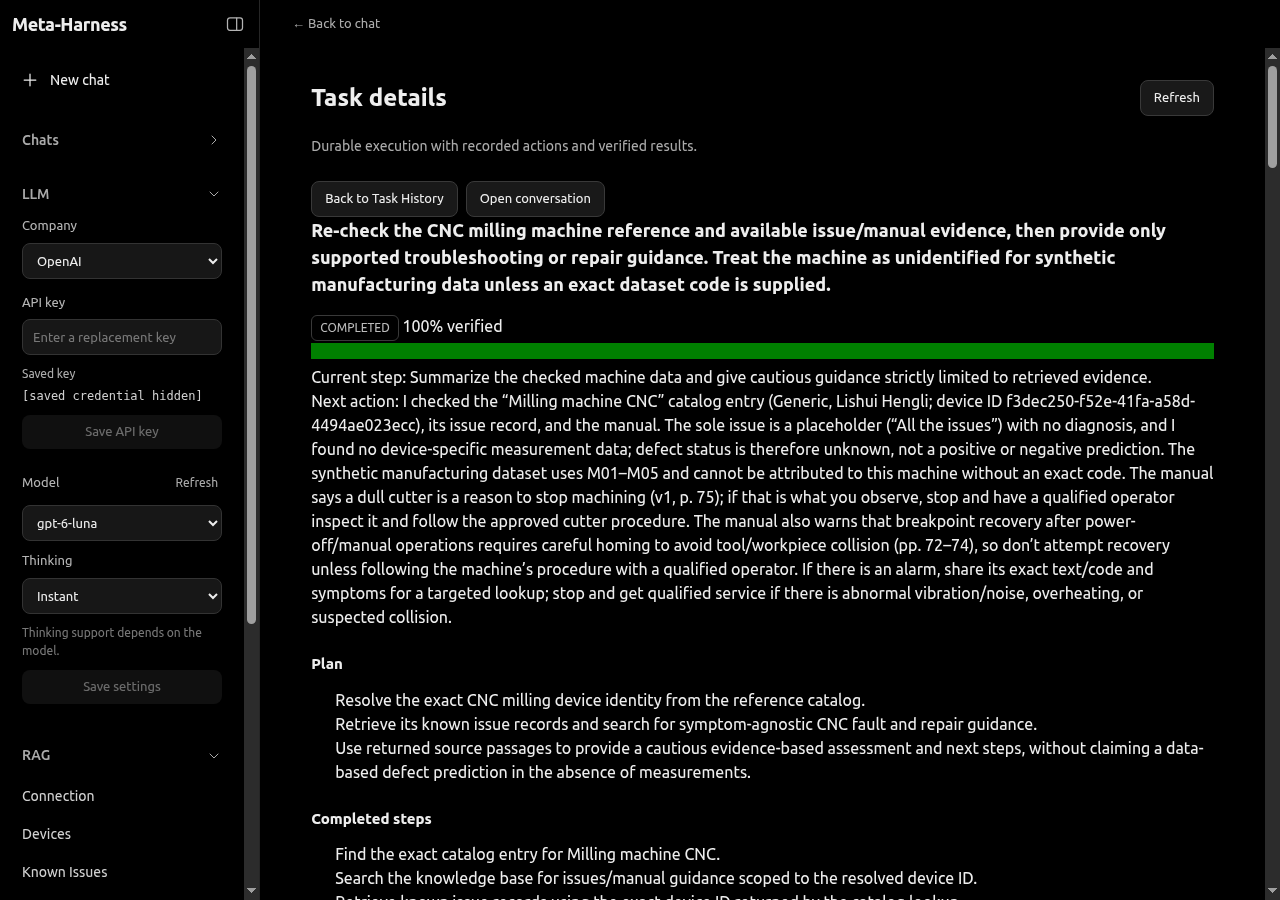
\includegraphics[width=.94\linewidth,trim=300bp 510bp 45bp 85bp,clip]{screenshots/task-details.png}\captionof{figure}{Detail from a genuine task-detail capture. This recorded CNC example illustrates the actual controls, not a ZSK diagnosis; its verified predicates do not certify industrial correctness.}\end{center}
\source{\path{ui/src/components/tasks/tasks-workspace.tsx}; \path{ui/src/components/chat/task-feedback.tsx}; \path{ui/src/components/rag/management.tsx}; \path{ui/src/App.tsx}; service READMEs and \path{docs/OPERATIONS.md}.}
